\documentclass[sigconf]{acmart}

\usepackage{graphicx}
\usepackage{hyperref}
\usepackage{todonotes}

\usepackage{endfloat}
\renewcommand{\efloatseparator}{\mbox{}} % no new page between figures

\usepackage{booktabs} % For formal tables

\settopmatter{printacmref=false} % Removes citation information below abstract
\renewcommand\footnotetextcopyrightpermission[1]{} % removes footnote with conference information in first column
\pagestyle{plain} % removes running headers

\newcommand{\TODO}[1]{\todo[inline]{#1}}

\begin{document}
\title{Using Big Data for Fact Checking}

\author{Karthik Vegi}
\affiliation{%
  \institution{Indiana University Bloomington}
  \streetaddress{2619 East 2nd Street, Apt 11}
  \city{Bloomington, IN 47401} 
  \country{USA}}
\email{kvegi@iu.com}


% The default list of authors is too long for headers}
\renewcommand{\shortauthors}{kvegi}


\begin{abstract}
In this data age, the sheer volume of data makes it impossible to know what is truth and what is not. Politicians are often misconstruing facts to improve their candidacy. Scientists and advertisers are making false claims to gain business advantage.  The more the false claims penetrate into the internet, especially social media, the more chances are that it is believed to be true. We show how Big Data techniques can be used to spot fake news, false claims made by politicians, advertisers, and scientists.
\end{abstract}

\keywords{i523, hid231, big data, veracity, fact check, data accuracy}

\maketitle

\section{Introduction}

{\em Big Data} is playing a crucial role in building a smarter planet. Each and every action that we take leaves a digital footprint. Big Data is lending a great helping hand to crunch this data and make smarter decisions. ``{\em Big Data} is at the heart of the smart revolution. It is already completely transforming the way we live, find love, cure cancer, conduct science, improve performance, run cities, and countries and operate business'' \cite{Marr2015}.  \\
Analyzing data in this digital era where data can come from multiple sources involves reading data from different systems in different formats with different contextual meanings. The data extracted from multiple systems can often contradict each other. It could be biased towards a business or a particular entity. Multiple sources also mean conflicting and outdated information which makes it highly inaccurate \cite{Berti-Equille2016}. \\
Validation of facts became a major issue with the recent U.S. election of 2016 where the candidates from both the democratic and republic parties used a lot of factual statements in the debates to put their candidacy and party in a better position. These factual statements if not validated might give a false edge to the party thus having an effect on the entire nation. While some people take these statements with a pinch of salt, a large set of population often believes it to be true and end up voting for party purely based on the claims made by the respective candidates \cite{www-forbes2}. With so many data sources like social media, print media, and the internet, it is not easy to validate and spot fake news. We need to take the help of the technological advances in {\em Big Data} and {\em Artificial Intelligence} to handle this problem.\\ 
Data inconsistencies with respect to the sources, interpreting the data out of the context, obsolete data and data that is highly modified from the original are all data veracity problems \cite{Berti-Equille2016}. ``Fake news and fact-checking is clearly a data veracity problem. Veracity refers to several quality dimensions related to repairing data inconsistencies and fixing other data quality problems such as duplicates, missing or incomplete data'' \cite{Berti-Equille2016}.

\section{Fact Checking as a Big Data Problem}
Often veracity is not just about data quality, it is about data understandability. Fake news is understandable and we can make great sense out of it by careful analysis \cite{www-forbes2}. The data veracity problem in {\em Big Data} meets the fake news problem at the juncture called {\em Misinformation Dynamics} where the emphasis is not just on the inaccuracy because of an accident, but on the data quality as a whole \cite{www-forbes2}. Fake news is often intentional and moreover, it is not static but dynamic \cite{www-forbes2}.  \\
One straightforward way to understand and account for the reliability of the sources is to formulate a voting algorithm that labels the source system in which the data item resides thus evaluating the accuracy of the data \cite{www-forbes1}. The problem with this approach is that it is too simple and also it doesn't take into account the other factors such as the data lineage of each source \cite{www-forbes1}. This means that if multiple sources of the data are all derived from another source which is inaccurate, we are wrongly labeling the data source \cite{www-forbes1}. \\ 
The social networking giants like Facebook and Twitter faced this problem and a lot of fingers were pointed at them for acting as a medium for spreading fake news. Facebook took the initiative to tackle the problem head-on by implementing an option where the users can flag the story as either true or false \cite{www-forbes2}. The more false votes s story garners, the less likely it appears on the news feed along with a warning message to the users mentioning that a lot of users have reported the story as false \cite{www-forbes2}. The problem with this approach is that we are giving people a chance to alter the truth, also making everyone believe that anything that is not flagged is true which might not always be the case \cite{www-forbes2}. \\ 
In order to solve this problem in a more efficient way, we could combine {\em Big Data} and {\em Artificial Intelligence} techniques that eradicate the possible human-generated errors \cite{www-forbes2}. {\em Google} came up with a new method of scoring web pages based on the accuracy of the facts in which the algorithm assigns documents a trust score taking the context into account, which feeds the overall scoring to determine the search rank without solely relying on the links \cite{www-forbes2}. \\
While the social networking giants have a huge role to play in identifying fake news, each individual should take personal responsibility to check the validity of the data using online tools at their disposal rather than believing it blindly. 

\section{Big Data Techniques for fact checking}

\subsection{Recommendation Based Approaches}
Recommendation based approaches take the help of the community to determine the accuracy and quality of the sources \cite{Berti-Equille2016}. The reputation of the sources increases as more people agree that the source is reliable \cite{Berti-Equille2016}. These methods clearly have their shortcomings as people can be influenced by third-party agencies to improve the trustworthiness of certain sources \cite{Berti-Equille2016}.

\subsection{Content Based Approaches}
Content based approaches work by coming up with a score to compute the trust of a source and validates the belief of the claims it is making to generate a belief score \cite{Berti-Equille2016}. The trustworthiness of the source now becomes a function of the trust score and the belief score \cite{Berti-Equille2016}. This is not a one time process but the function runs over and over to continuously update the source quality \cite{Berti-Equille2016}. A few probabilistic methods are added to this function to improve the accuracy of the score which extends the algorithm beyond just trust and belief \cite{Berti-Equille2016}. \\ In one such application, the truth discovery problem is transformed into a probabilistic inference model \cite{Zhao2014}. An iterative algorithm is proposed which computes the posterior distribution of all the values of the sources and finds the one with the maximum probability \cite{Zhao2014}. The model derives all the possible values reported by the sources and the conflicting values in the data streams and then calculates a score \cite{Zhao2014}. \\
Figure \ref{fig:Fig1} illustrates the content based approach for truth discovery in data streams. As there can be heterogeneous sources, first a semantic mapping is employed for the values provided by various sources such that the values for truth discovery are consistent \cite{Zhao2014}. Taking an example, the weather conditions that imply the same meaning such as {\em rainy} and {\em wet} are considered to be the same in truth discovery \cite{Zhao2014}. The same way, {\em partly sunny} and {\em cloudy} are considered as {\em clear} weather condition \cite{Zhao2014}. \\
``At each time {\em i}, the system collects a set of conflicting
values for entity {\em v} as {\em V} = $\left\{{v1,v2,...,vk}\right\}$ from multiple data sources. Next, the system resolves the conflicts and discovers the true value {\em v} in {\em V} based on the current data uncertainty and source quality. Then, the system updates the data uncertainty and source quality based on the inferred value {\em v} and conflicting values {\em V}'' \cite{Zhao2014}.

\begin{figure}
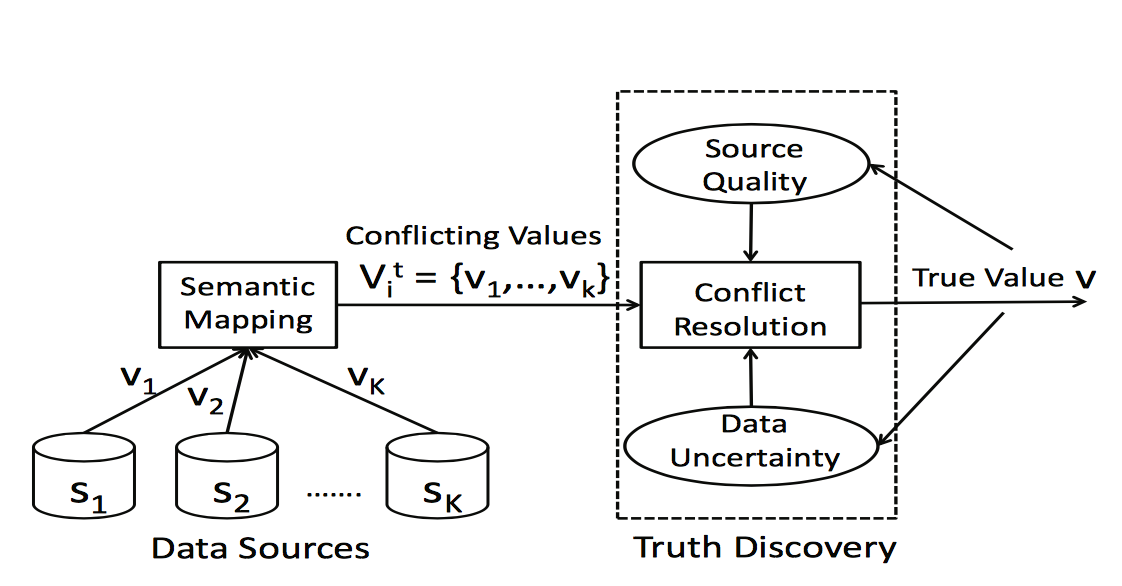
\includegraphics[width=1.0\columnwidth]{images/fig1.png}
\caption{Truth Discovery In Data Streams \cite{Zhao2014}}
\label{fig:Fig1}
\end{figure}

\subsection{Evidence Based Approaches}
Evidence based approaches augment the content based approaches by relying on evidence, context and prior knowledge about the data sources \cite{Berti-Equille2016}. Data provenance information may be used in truth discovery computation, as well as external information about the context, the sources, the data or user network \cite{Berti-Equille2016}. This involves checking the dynamics of information in the network and recomputing the truth discovery accordingly \cite{Berti-Equille2016}. Not every industry has a separate budget for research which makes evidence based approaches a viable option only for big organizations.

\section{Real-time Fact Checking}
In this digital age, fact checking makes more sense when it is done in real time. Politicians and media houses use inaccurate facts and make claims and get away with them in real time, but the new fact-checking tools can often expose claims that are invalid and inaccurate \cite{Hassan2015}.  The number of active fact-checking websites has been growing immensely, from about 44 in 2014 to about 114 currently \cite{Hassan2015}. \\
The delay window between the time when a claim is made and the time when the claim is checked for truth has to be as less as possible as fact checking often takes longer time than traditional journalism \cite{Hassan2015}. This gives enough time for the politicians and other people to make a claim and get away with it \cite{Hassan2015}.

\subsection{ClaimBuster}
{\em ClaimBuster} is a system that is built for real-time fact checking using the techniques of natural language processing and machine learning combined with database queries \cite{Claimbuster2017}. Although the complete system is still in works, some components of the system are already in use \cite{Claimbuster2017}.\\
Figure \ref{fig:Fig2} shows the system architecture of {\em ClaimBuster}. The {\em claim monitor} integrates the various data sources and feeds them into the system \cite{Claimbuster2017}. The {\em claim spotter} picks the claims that could potentially be checked for accuracy and reads in the relevant text from the data sources \cite{Claimbuster2017}. The {\em claim matcher} finds all the matching data sources that which mention the same claim in different ways \cite{Claimbuster2017}. The {\em claim checker} verifies them against external information from the internet to compute the accuracy of the claim \cite{Claimbuster2017}. The {\em fact-checker reporter} validates the claims against the facts gathered from {\em claim matcher} and compiles the accuracy report to publish them through sources like a website, a twitter account, or a slack-bot \cite{Claimbuster2017}. \\
In this way, the {\em ClaimBuster} gives every fact a score between 0 to 1, where a score closer to 1 is more accurate \cite{Claimbuster2017}. The model was well trained by using thousands of actual data from general election debates that has been manually fact-checked by humans \cite{Claimbuster2017}. The accuracy of the model was measured between 74 and 79 \cite{Claimbuster2017}. The system was put to use in real-time for the 2016 U.S. presidential election debates and the results showed a high match between {\em ClaimBuster} and journalists who checked for the accuracy of the claims \cite{Claimbuster2017}.  

\begin{figure}
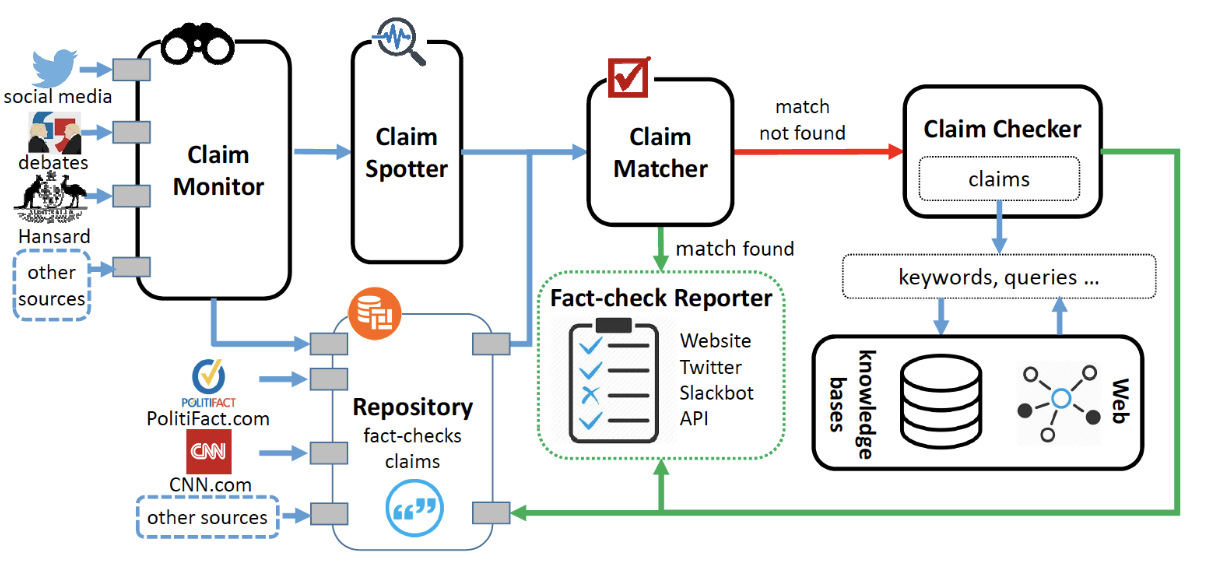
\includegraphics[width=1.0\columnwidth]{images/fig2.png}
\caption{System architecture of ClaimBuster \cite{Claimbuster2017}}
\label{fig:Fig2}
\end{figure}

\section{Conclusion}

{\em Big Data} coupled with {\em Artificial Intelligence} and {\em Machine Learning} can tackle the fact checking problem more efficiently. Rather than working in silos, the social networking giants and the search engine giants should work together with researchers to improve the existing system. This ensures that there are no loose ends with respect to the accuracy of the data. This is important because there is always a disconnect between data sources and not everybody has control and access to data that somebody else owns.
    
\begin{acks}

The author would like to thank Dr. Gregor von Laszewski and the teaching assistants for their support and suggestions in writing this paper.

\end{acks}

\bibliographystyle{ACM-Reference-Format}
\bibliography{report} 

\end{document}
